
\subsection{Metodología experimental}


{\color{red}
    En cuanto a la partición de los datos, se ha realizado una división entrenamiento-test con una proporción del 70\% y 30\%, respectivamente. Esta separación se ha llevado a cabo a nivel de \textit{trial}, evitando separar ventanas pertenecientes al mismo ensayo entre ambos conjuntos.

    La selección del conjunto de test no se ha realizado de forma aleatoria, sino utilizando los últimos \textit{trials} de cada sujeto y día. Esta decisión se basa en la hipótesis de que los sujetos presentan una mejora progresiva en el control de la imaginación motora a lo largo de la sesión, lo que permite evaluar el modelo en condiciones más estables.

    Finalmente, no se aplicaron técnicas adicionales de filtrado o procesamiento sobre las señales \acrshort{eeg}.
}


\subsubsection{Variables del estudio}

En este trabajo se realiza un análisis comparativo entre las arquitecturas \textit{EEGNet}, \textit{ShallowConvNet} y \textit{DeepConvNet}. Para ello, se han definido cuatro estrategias de entrenamiento con el objetivo de evaluar cómo se adapta cada modelo a diferentes usuarios, sesiones y condiciones experimentales.

Las tareas de imaginación motora consideradas son la imaginación de movimiento y la imaginación de parada. En la primera, el sujeto realiza un esfuerzo mental activo orientado a iniciar o mantener el movimiento del exoesqueleto. En la segunda, el sujeto realiza un esfuerzo mental activo orientado a detener dicho movimiento.

Las estrategias de entrenamiento seleccionadas se basan en los paradigmas descritos previamente en la sección \ref{sec:metodos_entrenamiento}.

\paragraph*{Entrenamiento intra sesión}

En esta estrategia se utilizan únicamente los datos de una sesión concreta y de un único usuario. Los ensayos de dicha sesión se dividen en conjuntos de entrenamiento y validación siguiendo una proporción del 70\% y 30\%, respectivamente. Para la validación se emplean siempre los últimos ensayos de la sesión.

Esta elección se basa en la hipótesis de que los sujetos pueden presentar una mejora progresiva en el control de la imaginación motora a lo largo de la sesión. Por tanto, evaluar el modelo sobre los últimos ensayos permite analizar su rendimiento en una fase potencialmente más estable de la tarea.

\paragraph*{Entrenamiento entre sesiones}

En este caso, el modelo se entrena utilizando los datos de las sesiones anteriores del mismo usuario. A estos datos se añaden los ensayos de entrenamiento de la sesión actual, manteniendo la misma división del 70\% para entrenamiento y 30\% para validación.

Esta estrategia permite evaluar si la información acumulada de sesiones previas mejora la adaptación del modelo a una nueva sesión del mismo usuario.

\paragraph*{Entrenamiento entre usuarios}

En esta estrategia se genera inicialmente un modelo general entrenado con los datos del resto de usuarios, excluyendo al usuario objetivo. Posteriormente, dicho modelo se ajusta mediante \textit{fine-tuning} utilizando los datos de entrenamiento de la sesión actual del usuario objetivo, manteniendo la misma proporción de entrenamiento y validación descrita anteriormente.

Este proceso se repite para todas las sesiones del usuario, generando un nuevo modelo adaptado para cada una de ellas. El objetivo de esta estrategia es analizar si un modelo preentrenado con datos de otros usuarios puede transferir conocimiento útil al usuario objetivo.


\paragraph*{Entrenamiento continuo}

El entrenamiento continuo sigue un esquema similar al entrenamiento entre usuarios, partiendo también de un modelo general entrenado con los datos del resto de usuarios. Sin embargo, en lugar de generar un nuevo modelo independiente para cada sesión, el modelo se conserva entre sesiones y se reentrena progresivamente con los datos disponibles de la sesión actual.

De este modo, el modelo incorpora de forma acumulativa la información del usuario objetivo, partiendo de un conocimiento inicial obtenido a partir del resto de usuarios y adaptándose gradualmente a sus sesiones sucesivas.


    {\color{red}
        \subsubsection{Estrategia de entrenamiento}\label{sec:estrategia_entrenamiento}

        epochs

        batch size

        callbacks:

        early stopping

        reduce LR

        función de pérdida

        métrica (accuracy)




        \subsubsection{Evaluación}


        validación cruzada

        pseudo-online

        explicar qué significa pseudo-online
    }


\subsection{Infraestructura Experimental}\label{sec:infraestructura_exp}

El elevado numero de ejecuciones requeridas para el estudio, hizo que, durante las etapas iniciales, se tomara la decisión de enfocar el proyecto de manera horizontal, preparando una base de ejecución sobre la cual modificar facilmente todo lo necesario para cada ejecución y permitiendo ejecutar multiples experimentos de manera secuencial.

Para lograr esto, se ha definido un pipeline de ejecución que permite realizar múltiples experimentos de forma iterativa y automatizada. Este pipeline está compuesto por distintos módulos encargados de gestionar el preprocesamiento de los datos, la configuración de los modelos, el entrenamiento y la evaluación de los mismos.

Con el objetivo de facilitar la reproducibilidad y la exploración sistemática de parámetros, el código se ha estructurado como un microframework que permite modificar de forma sencilla las variables de estudio, así como controlar la ejecución de los experimentos.

Para organizar la ejecución, se ha definido una estructura jerárquica en tres niveles:

\begin{itemize}
    \item \textbf{Experimento}: nivel superior que agrupa el conjunto completo de configuraciones evaluadas. Un experimento consiste en la ejecución sistemática de múltiples combinaciones de parámetros.
    \item \textbf{Iteración}: cada una de las ejecuciones individuales del pipeline dentro de un experimento, asociada a una combinación específica de parámetros (arquitectura, método de entrenamiento y tipo de tarea).
    \item \textbf{Entrenamiento}: nivel más bajo de la jerarquía, correspondiente al entrenamiento y evaluación de un modelo para un usuario y sesión concretos dentro de una iteración.
\end{itemize}

De este modo, cada experimento está compuesto por múltiples iteraciones, y cada iteración incluye varios entrenamientos, uno por cada usuario y sesión del dataset.
Los experimentos se definen mediante la combinación de distintos parámetros, entre los que destacan el tipo de tarea, la arquitectura del modelo y el método de entrenamiento. Para cada combinación se ejecuta una iteración independiente

En cada iteración, el sistema inicializa los parámetros de entrenamiento y carga el conjunto de datos correspondiente al tipo de tarea. A continuación, se ejecuta el método de entrenamiento seleccionado, en el que se itera sobre los distintos usuarios y sesiones disponibles en el dataset. Para cada caso, se inicializa el modelo, se realiza el entrenamiento y se evalúa su rendimiento.

Finalmente, los resultados obtenidos, junto con los parámetros utilizados, se almacenan de forma estructurada en una base de datos relacional usando el motor de DuckDB, permitiendo su posterior análisis. Un ánalisis detallado del esquema de la base de datos se presenta en el anexo \ref{sec:db_schema}.

Este proceso permite realizar un gran número de experimentos de manera secuencial y facilita el posterior estudio de los resultados obtenidos por cada combinación de parámetros definida.

La Figura \ref{fig:pipeline_general} resume la organización jerárquica del pipeline experimental.

\begin{figure}[htbp]
    \centering
    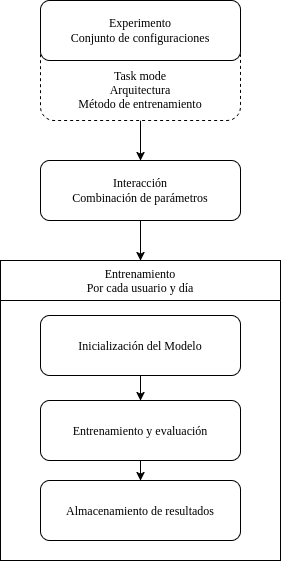
\includegraphics[width=0.45\textwidth]{img/diagrama_pipeline.drawio.png}
    %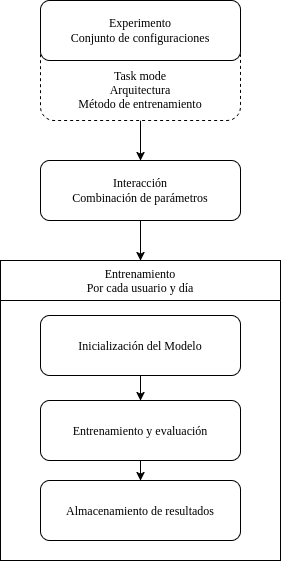
\includegraphics[height=\dimexpr\pagegoal-\pagetotal-\baselineskip\relax,width=\textwidth,keepaspectratio]{img/diagrama_pipeline.drawio.png}
    \caption{Pipeline experimental}
    \label{fig:pipeline_general}
\end{figure}








{\color{red}
\subsubsection{Diseño de experimentos}

combinaciones de parámetros
nº de ejecuciones
cómo comparas resultados

Esto lo iba a poner, ahora no lo tengo claro, pero lo dejo aquí para no olvidarlo
}
